\documentclass[a5paper,titlepage,10pt,openany]{scrbook}
\usepackage[a5paper,backref]{hyperref}
\usepackage[papersize={148.5mm,215mm},twoside,bindingoffset=0.5cm,hmargin={2cm,2cm},
				vmargin={2cm,2cm},footskip=1.1cm,driver=dvipdfm]{geometry}
\usepackage{palatino}
\usepackage[utf8]{inputenc}

\usepackage{pstricks}
\usepackage{graphicx}
\usepackage[bahasa]{babel} 
\usepackage{lettrine}
\usepackage{pifont}
\usepackage{enumitem}
\usepackage{wrapfig}
\usepackage{indentfirst}
\usepackage{parcolumns}
\usepackage[titles]{tocloft}
\usepackage{longtable}
\usepackage{microtype}
\usepackage{hyphenat}
%\usepackage[raggedright]{titlesec}
%\usepackage{titletoc}


\renewcommand{\cftchapfont}{%
  \fontsize{9}{8}\selectfont
}

\makeatletter
\renewcommand{\@pnumwidth}{1em} 
\renewcommand{\@tocrmarg}{1em}
\makeatother

\author{Lingkungan St. Petrus Maguwo}
\title{Warta Iman}
\setlength{\parindent}{1cm}
\psset{unit=1mm}

\makeatletter
\renewcommand{\@makeschapterhead}[1]{%
  {\parindent \z@ \centering \normalfont
    \interlinepenalty\@M \Large \bfseries #1\par\nobreak \vskip 20\p@ }}
\renewcommand{\section}{\@startsection {section}{1}{\z@}%
                                   {-3.5ex \@plus -1ex \@minus -.2ex}%
                                   {2.3ex \@plus.2ex}%
%                                   {\normalfont\normalsize\bfseries\centering}}
                                   {\normalfont\normalsize\bfseries}}
\renewcommand\subsection{\@startsection{subsection}{2}{\z@}%
                                     {-3.25ex\@plus -1ex \@minus -.2ex}%
                                     {1.5ex \@plus .2ex}%
                                     {\normalfont\normalsize\bfseries}}
\renewcommand\subsubsection{\@startsection{subsubsection}{3}{\parindent}%
                                    {3.25ex \@plus1ex \@minus.2ex}%
                                    {-1em}%
                                    {\normalfont\normalsize\bfseries}}

\makeatother

\makeatletter  % Allow the use of @ in command names
\long\def\@makecaption#1#2{%
  \vskip\abovecaptionskip
  \sbox\@tempboxa{{#1#2}}%
  \ifdim \wd\@tempboxa >\hsize
    {#1#2\par}
  \else
    \hbox to\hsize{\hfil\box\@tempboxa\hfil}%
  \fi
  \vskip\belowcaptionskip}
\makeatother   % Cancel the effect of \makeatletter

\newcommand{\chap}[1]{%
    \chapter*{#1}
	\addcontentsline{toc}{chapter}{#1}
    }

\newcommand{\sumber}[1]{%    
	\begin{flushright}
	{\emph{#1}}
	\end{flushright}
}
\newcommand{\qti}[1]{%    
	\begin{quote}
	{\emph{#1}}
	\end{quote}
}

\hyphenation{sa-u-da-ra-ku}
\hyphenation{ke-ri-ngat}
\hyphenation{je-ri-tan}
\hyphenation{hu-bung-an}
\hyphenation{me-nya-dari}
\hyphenation{Eng-kau}
\hyphenation{ke-sa-lah-an}
\hyphenation{ba-gai-ma-na}
\hyphenation{Tu-han}
\hyphenation{di-per-ca-ya-kan}
\hyphenation{men-ja-uh-kan}
\hyphenation{bu-kan-lah}
\hyphenation{per-sa-tu-kan-lah}
\hyphenation{ma-khluk}
\hyphenation{Sem-buh-kan-lah}
\hyphenation{ja-lan}
\hyphenation{mem-bu-tuh-kan}
\hyphenation{be-ri-kan-lah}
\hyphenation{me-ra-sa-kan}
\hyphenation{te-man-ilah}
\hyphenation{mem-bi-ngung-kan}
\hyphenation{di-ka-gum-i}
\hyphenation{ta-ngis-an-Mu}
\hyphenation{mi-lik-ilah}

\renewcommand{\figurename}{~}
\renewcommand\thefigure{~}

\setlist{noitemsep}
\renewcommand{\thesection}{\Alph{section}}

\begin{document}
\thispagestyle{empty}
\thispagestyle{empty}
\newcommand{\edisi}[1]{%
\DeclareFixedFont{\PT}{T1}{ppl}{b}{}{0.7in}
\DeclareFixedFont{\PTit}{T1}{ppl}{b}{it}{0.7in}
\DeclareFixedFont{\PTsmall}{T1}{ppl}{b}{it}{0.25in}
\DeclareFixedFont{\PTsmaller}{T1}{ppl}{b}{it}{0.175in}
\DeclareFixedFont{\PTsmallest}{T1}{ppl}{b}{it}{0.15in}

\begin{pspicture}(14cm,2cm)
\rput[rb](10.35cm,3cm){\PTsmallest {#1}}
\rput[lb](-2cm,1.5cm){\PT {WARTA IMAN}}
\rput[lb](0cm,0.5cm){\PTsmall {Lingkungan St. Petrus Maguwo}}
\end{pspicture}%
}

\newcounter{kgkcounter}[chapter]
\renewcommand{\thekgkcounter}{\arabic{kgkcounter}. }
\newcommand{\kgk}[1]{\refstepcounter{kgkcounter}\textbf{\flushleft \textbf{\thekgkcounter #1}}\\}

\newcommand{\kutipan}[1]{%
\noindent{\framebox{\parbox{10cm}{\centering\emph{#1}}}}}

\edisi{November 2011}

%\vspace{1cm}

\begin{center}
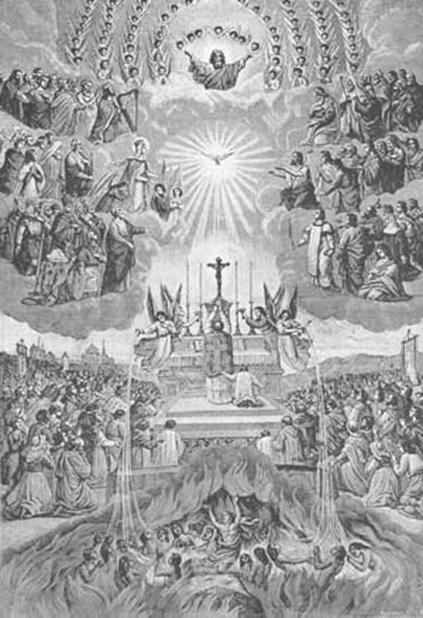
\includegraphics[scale=0.85]{gambar/purgatory2.jpg}
\end{center}

%\vspace{1cm}

\begin{center}
{\PTsmaller {Kasih, kerendahan hati, dan menurut pada kehendak Allah }}
\end{center}

\setlength{\parindent}{1cm}
\pagestyle{plain}
\chap{Tujuh pesan terakhir Yesus}

\section{Pesan terakhir yang penuh makna}
Kalau seseorang yang kita kasihi meninggal, maka kita mencoba mengingat pengalaman-pengalaman bersama dengan orang tersebut, baik pengalaman suka
maupun duka. Namun, terutama kita mencoba mengingat apa yang diucapkan pada
saat-saat menjelang ajalnya, karena pesan pada saat-saat terakhir adalah
penting dan penuh makna.

Dalam tulisan ini, maka kita akan melihat tujuh pesan Yesus yang diucapkan-Nya
pada saat Dia tergantung di kayu salib, saat-saat akhir hidup-Nya. Dari pesan
terakhir ini, kita akan dapat menangkap hal-hal yang terpenting yang ingin
disampaikan-Nya kepada kita. Tujuh pesan Yesus terdiri dari:
\begin{enumerate}
\item Luk 23:34 "Ya
Bapa, ampunilah mereka, sebab mereka tidak tahu apa yang mereka perbuat."; 
\item Luk 23:43 "Aku berkata kepadamu, sesungguhnya hari ini juga engkau akan ada
bersama-sama dengan Aku di dalam Firdaus." 
\item Yoh 19:26-27 "Ibu, inilah,
anakmu!" dan "Inilah ibumu!"; 
\item Mar 15:34 "Allahku, Allahku, mengapa Engkau
meninggalkan Aku?"; 
\item Yoh 19:28 "Aku haus!"; 
\item Yoh 19:30 "Sudah selesai";
\item Luk 23:46 "Ya Bapa, ke dalam tangan-Mu Kuserahkan nyawa-Ku."
\end{enumerate}

Dari pesan ini, kita melihat bagaimana Yesus ingin membawa keselamatan bagi
semua orang dengan memberikan pengampunan kepada umat manusia, sehingga manusia
dapat bersatu dengan Allah di dalam Kerajaan Sorga, sama seperti Yesus membawa
pencuri di sebelah kanan-Nya ke Firdaus. Bagaimana cara untuk mencapai Kerajaan
Sorga? Yesus menunjukkan agar kita dapat menerima Maria sebagai bunda kita,
senantiasa berharap pada Allah dalam kesulitan, haus akan jiwa-jiwa untuk
diselamatkan, serta terus setia terhadap panggilan kita sampai akhir hayat
kita, sampai tiba saatnya kita menyerahkan nyawa kita kepada Bapa dan kemudian
memulai kehidupan baru di dalam Kerajaan Sorga.

\subsection{Luk 23:34 "Ya Bapa, ampunilah mereka, sebab mereka tidak tahu apa yang
mereka perbuat."}

Pada saat Yesus tergantung di kayu salib, di tahta-Nya yang dipandang hina oleh
banyak orang, Dia melihat dengan jelas drama kehidupan kehidupan manusia, mulai
dari serdadu yang kejam, murid-muridnya yang pengecut, kaum Farisi yang iri
hati, orang-orang yang tidak melakukan apapun ketika mereka melihat
ketidakadilan. Di kayu salib dan juga dalam permenungan-Nya di taman Getsemani,
Kristus juga melihat dosa-dosa seluruh umat manusia, mulai dari Adam dan Hawa
sampai manusia terakhir. Ini berarti Dia juga melihat semua dosa kita. Inilah
yang menyebabkan Yesus meneteskan keringat darah.

Jika kita berdoa dan melakukan perbuatan kasih di masa kini, kita
menemani dan menghibur Kristus pada saat Dia mengalami penderitaan di Taman
Getsemani. Kita mengikuti apa yang diperintahkan oleh Kristus sendiri, ketika
Dia mengatakan "Hati-Ku sangat sedih, seperti mau mati rasanya. Tinggallah di
sini dan berjaga-jagalah dengan Aku." (Mat 26:38). Jangan biarkan kita lengah
sehingga Kristus menegur kita dengan mengatakan "Tidakkah kamu sanggup berjaga-
jaga satu jam dengan Aku?" (Mat 26:40).

Bagaimana dengan pengetahuan manusia seperti kita? Kita dapat mempunyai
pengetahuan eksperimental atau kalau Tuhan menghendaki. Namun, menjadi
kodrat dari manusia untuk belajar secara bertahap. Pengetahuan manusia akan
Tuhan didapatkan secara bertahap. 

Dengan melihat kodrat manusia ini, Kristus berdoa "Ya Bapa, ampunilah mereka,
sebab mereka tidak tahu apa yang mereka perbuat." (lih. Luk 23:34). Kristus
tahu bahwa manusia memang berdosa karena dipengaruhi oleh kelemahan-
kelemahannya akibat dosa asal. Dengan demikian, apa yang diperbuat oleh manusia
bisa saja terjadi karena ketidaktahuannya. 

Namun tidak semua ketidaktahuan
mengakibatkan orang terbebas dari dosa. Ketidakketidaktahuan yang tak
terhindari (\textit{invincible ignorance}) membuat orang tidak berdosa, namun
ketidaktahuan yang disebabkan oleh ketidakpedulian orang itu sendiri (\textit{culpable
ignorance}) menyebabkan seseorang tetap bersalah. Rasul Petrus mengerti bahwa
orang-orang yang menyalibkan Yesus bertindak karena ketidaktahuan mereka,
sehingga dia mengatakan \textit{"Hai saudara-saudara, aku tahu bahwa kamu telah berbuat
demikian karena ketidaktahuan, sama seperti semua pemimpin kamu."} (Kis 3:17)

Bagaimana dengan kita yang telah menerima Kristus? Kita tidak mempunyai alasan
lagi bahwa kita tidak tahu. Oleh karena itu, tanggung jawab kita lebih berat,
karena barang siapa diberi banyak akan dituntut lebih banyak (lih. Luk 12:48).
Menyadari bahwa manusia dengan kekuatannya sendiri tidak dapat menjalankan
semua perintah Allah, Kristus menyediakan Diri-Nya sendiri untuk disalibkan,
sehingga rahmat yang berlimpah dapat mengalir kepada kita umat Allah. 

Bahkan
kesalahan-kesalahan yang dibuat umat Allah dapat dihapuskan dengan melakukan
pengakuan dosa. Dan kalau seseorang tidak mensyukuri dan menggunakan semua
kemudahan untuk mendapatkan pengampunan dosa, maka orang tersebut tidak lagi
mempunyai alasan apapun kalau sampai dia kehilangan keselamatan kekal.

\subsection{Luk 23:43 "Aku berkata kepadamu, sesungguhnya hari ini juga engkau
akan ada bersama-sama dengan Aku di dalam Firdaus."}

Seluruh
kehidupan-Nya ditujukan untuk mengemban misi ini, dan Kristus telah
melaksanakannya dengan sempurna. Bahkan sampai pada menjelang akhir wafat-Nya,
Dia tidak membuang kesempatan sedikitpun untuk menyelamatkan pencuri yang
disalibkan bersama-Nya.

Menjadi sesuatu yang umum, bahwa pada saat seseorang disalibkan, maka dia akan
menyumpahi orang yang menyalibkannya, bahwa menyumpahi dirinya, menyumpahi
Tuhan dan hari kelahirannya. 
Namun, dua pencuri yang disalibkan mendengarkan
seseorang yang disalib di tengah-tengah mereka mengatakan, "Ya Bapa, ampunilah
mereka, sebab mereka tidak tahu apa yang mereka perbuat." (Luk 23:34).

Pengampunan ini mendatangkan rahmat. Paling tidak salah satu dari pencuri ini
menyambut rahmat Allah. Bahkan ketika pencuri di sebelah kiri mengatakan
"\textit{Bukankah Engkau adalah Kristus? Selamatkanlah diri-Mu dan kami!"} (Luk 23:39),
maka pencuri di sebelah kanan Yesus menjawab 
\textit{"40 Tidakkah engkau takut, juga
tidak kepada Allah, sedang engkau menerima hukuman yang sama? 41  Kita memang
selayaknya dihukum, sebab kita menerima balasan yang setimpal dengan perbuatan
kita, tetapi orang ini tidak berbuat sesuatu yang salah."} (Luk 23:40-41)

Percakapan ini mungkin terlihat sepele. Namun, kita jangan melupakan bahwa
setiap kata yang keluar dari orang yang disalibkan adalah merupakan suatu
penderitaan, karena setiap tarikan nafas menjadi suatu siksaan. Pencuri di
sebelah kanan, yang menurut tradisi bernama Dimas, dalam keterbatasannya telah
memberikan nyawanya untuk Kristus, dan dia juga menaruh pengharapan di dalam
Kristus, sehingga dia memohon kepada Yesus \textit{"Yesus, ingatlah akan aku, apabila
Engkau datang sebagai Raja."} (Luk 23:42) Sungguh suatu ungkapan pengharapan dan
iman yang begitu sederhana dan dalam. 

Terhadap ungkapan iman dan kasih ini,
Yesus menjawab "Aku berkata kepadamu, sesungguhnya hari ini juga engkau akan
ada bersama-sama dengan Aku di dalam Firdaus." (Luk 23:43)

Mari, dalam Pekan Suci ini, kita bersama-sama merenungkan, bahwa kita yang
telah menerima baptisan sakramental, seharusnya mempunyai sikap seperti yang
ditunjukkan oleh Dimas, bahkan dituntut lebih. Mengapa? Karena kita telah
menerima rahmat Allah yang begitu istimewa dalam Sakramen Baptis, seperti: 
\begin{enumerate}[label=(\alph{enumi})]
\item rahmat pengudusan, 
\item menjadi anak-anak Allah dan dipersatukan dalam Tubuh
Mistik Kristus, 
\item menerima tiga kebajikan ilahi (iman, pengharapan dan
kasih), 
\item menerima tujuh karunia Roh Kudus seperti yang disebutkan di dalam
Yes 11:2-3 (kebijaksanaan, pengertian, nasihat, keperkasaan, pengenalan,
kesalehan, dan takut kepada Allah). 
\end{enumerate}

Dengan rahmat-rahmat ini kita dimampukan
untuk mengikuti perintah Kristus, yang menuntun kita kepada keselamatan kekal.

\subsection{Yoh 19:26-27 "Ibu, inilah, anakmu!" dan "Inilah ibumu!"}
Memandang dari kayu salib, Kristus melihat dua orang
yang dikasihi-Nya, yaitu Ibu-Nya, Bunda Maria dan murid-Nya yang terkasih,
rasul Yohanes. Dengan sisa-sisa nafas-Nya, Kristus memberikan pesan yang begitu
penting kepada kita, yaitu pesan ketika Kristus memandang Ibu-Nya dan murid-Nya
dan berkata "Ibu (RSV = \textit{Woman}), inilah, anakmu!.. dan inilah ibumu" (Yoh 19:26-
27). 

Kristus menyerahkan ibu-Nya kepada  kepada murid yang
dikasihi-Nya – tanpa nama, untuk menyatakan bahwa perintah ini ditujukan kepada
semua murid Kristus.
Sebaliknya Kristus juga menyerahkan murid-Nya untuk menjadi putera Bunda Maria.
Satu-satunya anak Maria memang tidak tergantikan, yaitu Kristus. Ini
berarti, Kristus menginginkan agar Bunda Maria turut berpartisipasi dalam karya
keselamatan Kristus dan memperlakukan seluruh umat beriman sebagai anaknya.

Suka atau tidak suka, Kristus menginginkan hal ini dan memberikan Maria sebagai
bunda bagi seluruh umat beriman. Kalau Kristus tidak berkeberatan untuk dididik
oleh Maria dan Maria dipandang baik oleh Kristus sebagai Bunda Allah, maka
siapakah kita yang memandang bahwa kita tidak perlu menghormati Bunda Maria,
bahkan ada yang menyingkirkan Bunda Maria dari kehidupannya? Apakah ada seorang
pria yang merasa bahwa pacarnya terlalu berlebihan karena dia menghormati
ibunya juga?

\subsection{Mrk 15:34 "Allahku, Allahku, mengapa Engkau meninggalkan Aku?"}
Di dalam penderitaan-Nya, Dia telah menunjukkan adanya suatu kepercayaan yang
kokoh akan rencana Allah. Perkataan Eli, Eli Lamasabakthani, merupakan
permulaan dari Mazmur 22, yang lengkapnya adalah sebagai berikut:
\begin{quote}
\scriptsize
\begin{enumerate}
     \item  Untuk pemimpin biduan. Menurut lagu: Rusa di kala fajar. Mazmur
     Daud. (22-2) Allahku, Allahku, mengapa Engkau meninggalkan aku? Aku
     berseru, tetapi Engkau tetap jauh dan tidak menolong aku.
     \item Allahku, aku berseru-seru pada waktu siang, tetapi Engkau tidak
     menjawab, dan pada waktu malam, tetapi tidak juga aku tenang.
     \item Padahal Engkaulah Yang Kudus yang bersemayam di atas puji-pujian
     orang Israel.
     \item Kepada-Mu nenek moyang kami percaya; mereka percaya, dan Engkau
     meluputkan mereka.
     \item Kepada-Mu mereka berseru-seru, dan mereka terluput; kepada-Mu
     mereka percaya, dan mereka tidak mendapat malu.
     \item Tetapi aku ini ulat dan bukan orang, cela bagi manusia, dihina oleh
     orang banyak.
     \item Semua yang melihat aku mengolok-olok aku, mereka mencibirkan
     bibirnya, menggelengkan kepalanya:
     \item "Ia menyerah kepada TUHAN; biarlah Dia yang meluputkannya, biarlah
     Dia yang melepaskannya! Bukankah Dia berkenan kepadanya?"
     \item Ya, Engkau yang mengeluarkan aku dari kandungan; Engkau yang
     membuat aku aman pada dada ibuku.
     \item Kepada-Mu aku diserahkan sejak aku lahir, sejak dalam kandungan
     ibuku Engkaulah Allahku.
     \item Janganlah jauh dari padaku, sebab kesusahan telah dekat, dan tidak
     ada yang menolong.
     \item Banyak lembu jantan mengerumuni aku; banteng-banteng dari Basan
     mengepung aku;
     \item mereka mengangakan mulutnya terhadap aku seperti singa yang
     menerkam dan mengaum.
     \item Seperti air aku tercurah, dan segala tulangku terlepas dari
     sendinya; hatiku menjadi seperti lilin, hancur luluh di dalam dadaku;
     \item kekuatanku kering seperti beling, lidahku melekat pada langit-
     langit mulutku; dan dalam debu maut Kauletakkan aku.
     \item Sebab anjing-anjing mengerumuni aku, gerombolan penjahat mengepung
     aku, mereka menusuk tangan dan kakiku.
     \item Segala tulangku dapat kuhitung; mereka menonton, mereka memandangi
     aku.
     \item Mereka membagi-bagi pakaianku di antara mereka, dan mereka
     membuang undi atas jubahku.
     \item Tetapi Engkau, TUHAN, janganlah jauh; ya kekuatanku, segeralah
     menolong aku!
     \item Lepaskanlah aku dari pedang, dan nyawaku dari cengkeraman anjing.
     \item Selamatkanlah aku dari mulut singa, dan dari tanduk banteng.
     Engkau telah menjawab aku!
     \item Aku akan memasyhurkan nama-Mu kepada saudara-saudaraku dan memuji-
     muji Engkau di tengah-tengah jemaah:
     \item kamu yang takut akan TUHAN, pujilah Dia, hai segenap anak cucu
     Yakub, muliakanlah Dia, dan gentarlah terhadap Dia, hai segenap anak
     cucu Israel!
     \item Sebab Ia tidak memandang hina ataupun merasa jijik kesengsaraan
     orang yang tertindas, dan Ia tidak menyembunyikan wajah-Nya kepada
     orang itu, dan Ia mendengar ketika orang itu berteriak minta tolong
     kepada-Nya.
     \item Karena Engkau aku memuji-muji dalam jemaah yang besar; nazarku
     akan kubayar di depan mereka yang takut akan Dia.
     \item Orang yang rendah hati akan makan dan kenyang, orang yang mencari
     TUHAN akan memuji-muji Dia; biarlah hatimu hidup untuk selamanya!
     \item Segala ujung bumi akan mengingatnya dan berbalik kepada TUHAN; dan
     segala kaum dari bangsa-bangsa akan sujud menyembah di hadapan-Nya.
     \item Sebab Tuhanlah yang empunya kerajaan, Dialah yang memerintah atas
     bangsa-bangsa.
     \item Ya, kepada-Nya akan sujud menyembah semua orang sombong di bumi,
     di hadapan-Nya akan berlutut semua orang yang turun ke dalam debu,
     dan orang yang tidak dapat menyambung hidup.
     \item Anak-anak cucu akan beribadah kepada-Nya, dan akan menceritakan
     tentang TUHAN kepada angkatan yang akan datang.
     \item Mereka akan memberitakan keadilan-Nya kepada bangsa yang akan
     lahir nanti, sebab Ia telah melakukannya.
\end{enumerate}
\end{quote}

Bagi umat Yahudi, kalau seseorang memulai kalimat pertama dari Mazmur, maka
berarti orang bermaksud untuk menyelesaikannya. Dan dalam kondisi tersalib,
sungguh tidak mungkin untuk menyelesaikan pengucapan keseluruhan Mazmur
tersebut. Ini berarti, bahwa kalimat pertama dari Mazmur 22 harus dimengerti
dalam konteks keseluruhan, yaitu untuk mempercayai dan menggantungkan segala
sesuatunya ke dalam tangan Bapa, yang pada akhirnya akan membawa kemuliaan, di
mana seluruh ujung bumi akan mengingat dan berbalik kepada Tuhan (lih. Mzm 22:
27). 

Ini adalah suatu pengajaran dari Kristus yang harus diikuti oleh seluruh
murid Kristus tentang bagaimana menaruh pengharapan di dalam Tuhan dalam
kondisi apapun. Cara dan sikap dalam menghadapi penderitaan adalah salah satu
perbedaan antara orang yang mengenal Kristus dan yang tidak mengenal Kristus.

Bahkan rasul Paulus mengatakan (Rom 5:3-5)
\begin{quote} 
\scriptsize
\begin{enumerate}
\setcounter{enumi}{2}

\item Dan bukan hanya itu saja. Kita malah bermegah
juga dalam kesengsaraan kita, karena kita tahu, bahwa kesengsaraan itu
menimbulkan ketekunan, \item  dan ketekunan menimbulkan tahan uji dan tahan uji
menimbulkan pengharapan. \item  Dan pengharapan tidak mengecewakan, karena kasih
Allah telah dicurahkan di dalam hati kita oleh Roh Kudus yang telah
dikaruniakan kepada kita." 
\end{enumerate}
\end{quote}

Kalau seseorang menjadi murid Kristus, maka dia akan mengikuti apa yang
dilakukan oleh Kristus, termasuk adalah cara menghadapi permasalahan dan
penderitaan. Karena dengan penderitaan-Nya, Kristus dapat memenangkan belenggu
dosa, maka dengan menyatukan segala penderitaan kita dengan Kristus, kita akan
memperoleh kemenangan, yaitu kemenangan yang menyelamatkan, yang mengantar kita
pada  kehidupan kekal. Kuncinya adalah menghadapi permasalahan dengan terus
bertekun dalam doa yang didasarkan iman, pengharapan dan kasih, seperti yang
dilakukan oleh Kristus.

Mungkin ada yang bertanya, kalau Yesus memang Tuhan, mengapa pada saat disalib,
Dia berdoa? Santo Thomas Aquinas
membahas tentang definisi doa, dimana dia mengatakan bahwa doa adalah membuka
keinginan kita kepada Tuhan, sehingga Dia dapat memenuhinya." Karena di
dalam Kristus (satu pribadi) ada dua kehendak, yaitu kehendak manusia dan
kehendak Tuhan, maka menjadi hal yang wajar, kalau Yesus berdoa karena Dia
mempunyai kodrat manusia. Sama seperti kita sebagai orang beriman, kita
menyatakan keinginan/ kehendak kita di hadapan Allah.

Alasan kedua adalah Yesus berdoa untuk kepentingan manusia. Yesus dapat saja
berdoa dalam hati, namun Dia ingin menunjukkan kepada kita bagaimana seharusnya
sebagai manusia kita berdoa, yaitu bahwa kita harus senantiasa tunduk kepada
kehendak Allah Bapa, meskipun di dalam situasi yang paling sulit sekalipun.

Yesus mengajarkan doa yang sempurna, yaitu doa Bapa Kami, yang terdiri dari
tujuh petisi (lih. Mt 6:9-13).
Yesus menunjukkan bahwa di dalam setiap percobaan, maka Tuhanlah yang menjadi
kekuatan dalam doa, seperti yang ditunjukkan oleh Yesus di dalam drama
penyaliban (Mt 27:46; Mk 15:34; Lk 23:46).
Yesus juga mengajarkan pentingnya untuk mengampuni orang yang bersalah kepada
kita, seperti yang ditunjukkan oleh Yesus dengan berdoa "Ya Bapa, ampunilah
mereka, sebab mereka tidak tahu apa yang mereka perbuat." (lih. Lk 23:34).
Dan masih begitu banyak contoh yang lain, yang menyebabkan pengikut Kristus
tahu bagaimana untuk berdoa, karena Tuhan sendiri – melalui Kristus – yang
menunjukkan kepada manusia bagaimana seharusnya berdoa.

Dengan demikian, maka kita dapat melihat bahwa doa Yesus di atas kayu salib
sungguh merupakan doa yang berpengharapan yang menyelamatkan dan memberikan
contoh bagi seluruh umat beriman.

\subsection{Yoh 19:28 "Aku haus!"}
Contoh apalagi yang ingin diberikan oleh Kristus sebelum dia menghembuskan
nafas-Nya yang terakhir ketika Dia mengatakan "Aku haus!"? Dikatakan di ayat
Yoh 19:28 bahwa perkataan Yesus "Aku Haus" adalah untuk memenuhi nubuat di
dalam Kitab Suci. Ini adalah pemenuhan dari Mzm 69:21 yang mengatakan "… dan
pada waktu aku haus, mereka memberi aku minum anggur asam." Dengan demikian,
pernyataan Yesus merupakan penegasan bahwa Yesus yang tersaliblah yang
dinubuatkan dalam Perjanjian Lama.

Memang dalam kodrat-Nya sebagai manusia, Yesus mengalami penderitaan dan
kehausan yang begitu sangat. Namun, kehausan dalam kapasitas yang lebih dalam
adalah kehausan untuk meyelamatkan jiwa-jiwa. Ini adalah drama pencarian Tuhan
akan manusia. Drama di mana Tuhan yang dari Sorga turun ke dunia untuk
menjangkau jiwa-jiwa yang tercerai berai. 

Kehausan ini mengingatkan kita akan
permintaan Yesus kepada wanita Samaria "Berilah Aku minum" (Yoh 4:7). Dan
percakapan ini pada akhirnya membawa keselamatan kepada wanita Samaria dan juga
orang-orang di kota tersebut. Keselamatan wanita Samaria dan orang-orang di
kota tersebut tidaklah cukup bagi Yesus, sehingga di atas kayu salib, Dia tetap
merasa kehausan, karena Dia ingin menjangkau seluruh umat manusia, ingin
menemukan dan mengantar seluruh umat manusia pada keselamatan dan pengetahuan
akan kebenaran (lih. 1Tim 2:4)

Karena Tuhan senantiasa dalam pencarian akan manusia, maka sejak dari
Perjanjian Lama dikatakan "13 apabila kamu mencari Aku, kamu akan menemukan
Aku; apabila kamu menanyakan Aku dengan segenap hati, 14  Aku akan memberi kamu
menemukan Aku" (Yer 29:13-14) Inilah sebabnya ketika seseorang menyadari bahwa
dia memerlukan Tuhan, ketika seseorang melihat penderitaan dalam kacamata iman,
ketika seseorang menerima penderitaan dengan tabah, ketika seseorang mau
menyangkal dirinya dan memikul salibnya dan mengikuti Kristus, maka Tuhanlah
yang sebenarnya menjadi penggerak utama dari semuanya itu. Dalam drama
penyaliban, terutama perkataan Yesus bahwa Dia haus, kita menyaksikan akan
drama tentang Tuhan yang sungguh mencintai manusia dengan sehabis-habisnya.
Bagaimana tanggapan manusia? Bagaimana tanggapan kita?

\subsection{Yoh 19:30 "Sudah selesai"}
Setelah prajurit memberikan bunga karang yang telah dicelupkan pada anggur
asam, lalu Yesus meminumnya dan berkata "sudah selesai" (lih. Yoh 19:30). Kita
dapat melihat adanya tiga hal yang berkaitan dengan "sudah selesai". Di dalam
Kitab Kejadian, setelah Tuhan menyelesaikan penciptaan, maka pada hari ke
tujuh, Dia mengatakan "Ketika Allah pada hari ketujuh telah menyelesaikan
pekerjaan yang dibuat-Nya itu, berhentilah Ia pada hari
ketujuh dari segala pekerjaan yang telah dibuat-Nya itu." (Kej 2:2) 

Dalam konteks inilah Yesus mengatakan "sudah selesai" untuk menyatakan
bahwa Dia telah menyelesaikan pekerjaan yang diberikan oleh Bapa dengan
sempurna, bukan dengan keputusasaan dan kegetiran, namun dengan dasar kasih
yang sempurna. Inilah yang membuat persembahan Kristus di kayu salib dapat
menyenangkan hati Bapa -- yaitu karena didasarkan kasih yang sempurna.
Ini juga yang seharusnya mendorong kita dalam perjalanan kehidupan kita. Sama
seperti Rasul Paulus, kita juga ingin berlari ke tujuan untuk memperoleh
hadiah, yaitu panggilan Sorgawi dari Allah dalam Kristus Yesus (lih. Flp 3:14).

\subsection{Luk 23:46 "Ya Bapa, ke dalam tangan-Mu Kuserahkan nyawa-Ku."}
Kata yang terakhir dari Yesus setelah mengatakan "sudah selesai" adalah "Ya
Bapa, ke dalam tangan-Mu Kuserahkan nyawa-Ku". Dalam satu kalimat ini, kita
dapat melihat hubungan yang sungguh dalam dan tak terpisahkan antara Bapa dan
Putera. Bapa begitu mencintai manusia, sehingga Dia mengutus Putera-Nya yang
tunggal untuk menebus dosa dan menyelamatkan manusia (lih. Yoh 3:16). Kristus
datang ke dunia dan senantiasa melaksanakan kehendak Bapa. Dari umur duabelas
tahun, Kristus telah mengatakan bahwa Dia harus berada di dalam rumah Bapa-Nya
(Luk 2:49). Dalam seluruh karya-Nya, Kristus senantiasa melakukan apa yang
berkenan kepada Bapa (lih. Yoh 8:29). Sampai pada akhirnya, Kristus menyerahkan
nyawaNya ke dalam tangan Bapa (lih. Luk 23:46). Dengan kebebasan-Nya, Kristus
melakukan kehendak Bapa.

Bagaimana dengan kita? Bagaimana kita menggunakan kebebasan kita? Orang sering
salah dalam mengartikan kebebasan. Orang sering mengartikan kebebasan sebagai
"kebebasan dari" dan bukan "kebebasan untuk".
Kebebasan yang lebih menekankan "kebebasan dari" merupakan ekspresi akan
keinginan yang terbebas dari hal-hal yang dianggap mengikatnya, termasuk
tanggung jawab. Orang yang menginginkan kebebasan untuk minum minuman keras
tanpa mau dibatasi jumlahnya, cepat atau lambat akan menemukan bahwa dirinya
tidak lagi bebas. Dia akan terikat akan minuman keras, dan tidak lagi mempunyai
kebebasan untuk mengatakan tidak terhadap minuman keras. Dengan demikian, kita
dapat melihat bahwa mengumbar kebebasan tanpa adanya batasan yang jelas dapat
membuat manusia menjadi tidak bebas lagi. 

Mari, dalam Pekan Suci ini, kita merenungkan sejauh mana kita telah menggunakan
kebebasan kita. Apakah kita telah menggunakan kebebasan kita dengan
bertanggungjawab berdasarkan kebenaran dan kebaikan, sehingga dapat mengarahkan
kita kepada keselamatan diri kita maupun membantu keselamatan orang-orang di
sekitar kita? Jika kita telah mati dari dosa kita -- karena Sakramen Baptis --
yang kita terima, dan membuat kita dapat bangkit bersama Kristus, maka kita
juga harus mengikuti teladan Kristus. Kita dapat menyerahkan kebebasan kita
kepada Tuhan sehingga kita dapat semakin bebas untuk melaksanakan seluruh
perintah Tuhan.

\section{Melaksanakan tujuh pesan terakhir Yesus mengantar kita kepada keselamatan}

Dari pemaparan di atas, kita dapat melihat bahwa tujuh pesan terakhir Yesus
sungguh penuh makna yang mendalam. Kalau kita terus merenungkan pesan-pesan ini
sepanjang Pekan suci ini, maka kita akan semakin menghargai pengorbanan Yesus.
Apapun kondisi kita, di Pekan suci ini, Kristus menawarkan pengampunan kepada
kita semua. Bagi yang berdosa berat, segeralah mengaku dosa dan bagi yang
berjuang dalam kekudusan, teruslah berfokus pada tujuan akhir. Yesus
menginginkan agar semua manusia dapat sampai pada tujuan akhir, yaitu Sorga.
Tidak ada kata terlambat. Sejauh kita masih hidup dan bertobat, sama seperti
pencuri yang disalibkan di sisi kanan Yesus, maka Kristus akan memberikan janji
yang sama, yaitu keselamatan kekal.
Demikian pula, Kristus menyerahkan Bunda-Nya menjadi Bunda segenap umat
beriman, agar kita dapat memohon dukungan doanya agar dapat sampai kepada
keselamatan. Tujuan akhir ini juga harus dihadapi dengan pengharapan akan
Allah, sehingga pencobaan dan penderitaan tidak menjadikan kita perputus asa.
Dalam perjalanan kita menuju Sorga, kita juga harus mempunyai semangat untuk
membawa orang-orang di sekitar kita untuk memperoleh pengetahuan akan
kebenaran. Dan ini harus kita lakukan sampai akhir hidup kita, sampai tugas
kita selesai dan sampai kita menyerahkan nyawa kita ke dalam tangan Bapa.
Dengan menjalankan pesan Kristus ini, maka kita dapat mencapai tujuan akhir
dengan selamat.
Semoga Trihari Suci membawa kita pada permenungan yang lebih mendalam akan
misteri Paskah Kristus.

\sumber{Ditulis oleh: Stefanus Tay\\
Stefanus Tay telah menyelesaikan program studi S2 di bidang teologi di Universitas Ave Maria - Institute for Pastoral Theology, Amerika Serikat.}

\begin{center}
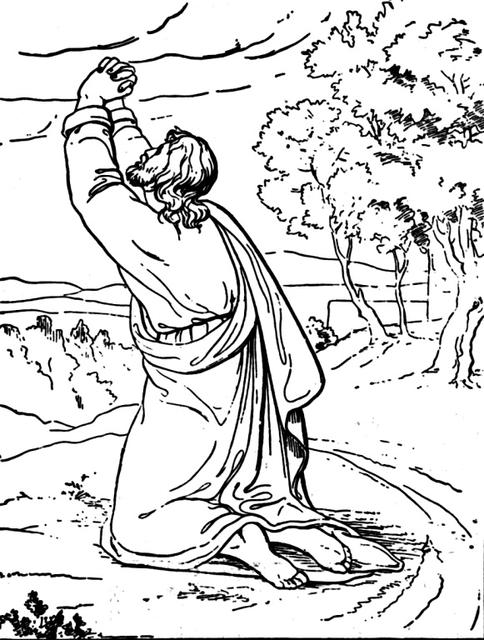
\includegraphics[scale=0.45]{gambar/jesus-praying.jpg}
\end{center}
\chap{Menciptakan Peluang}
\small
\noindent{ Dari Kejadian 45 : 5}

\begin{wrapfigure}[7]{r}{3.5cm}

\includegraphics[scale=0.5]{gambar/like.png}
\end{wrapfigure} 
\begin{quote}
\textit{``tetapi sekarang, janganlah bersusah hati dan janganlah menyesali diri, karena kamu menjual aku kesini, sebab untuk memelihara kehidupanlah Allah menyuruh aku mendahului kamu,''}
\end{quote}

Menurut Diana Kirschner, Ph.D., psikolog dan ahli komunikasi, rasa cemburu adalah suatu bentuk pemikiran negatif yang datang dari dalam diri sendiri. Melalui penelitian, terbukti bahwa rasa cemburu bisa berujung pada sakit hati, curiga, ledakan amarah, bahkan kemunduran kualitas dalam berhubungan. Tapi, mungkinkah rasa cemburu diubah menjadi sesuatu yang positif? Inilah salah satu caranya.

\textbf{Ketika rasa cemburu mulai merayapi pikiran,} sadari bahwa hal itu merupakan tanda betapa Anda sangat menyayangi pasangan. Daripada melelahkan diri dengan pikiran-pikiran negatif, cobalah untuk mendekati pasangan Anda dan katakan betapa sayangnya Anda kepadanya.

Di kehidupan ini kadang kita tidak tidak bisa memilih. \textbf{Suka atau tidak, kita harus belajar untuk menerima segala sesuatu apa adanya.} Kenyataan di depan kita adalah fakta tak terbantahkan dan kita tidak memiliki alternatif lain. \textbf{Jika hal seperti ini terjadi, bagaimana tindakan selanjutnya? Apakah kita harus arah dengan situasi yang ada?} Marilah kita belajar dari kehidupan tokoh alkitab perjanjian lama yang bernama Yusuf.

Yusuf adalah pemuda yang harus kehilangan kemerdekaan dan harkat sebagai orang merdeka karena dijual para saudaranya yang iri kepadanya. Berbagai pengalaman berat setelah itu pun harus ia alami. Namun, Yusuf tidak sudi menyerah. Dengan pertolongan Allah, ia berhasil mengubah semua rintangan di jalan kehidupannya sebagai kesempatan. Dalam beberapa tahun, ia akhirnya diangkat oleh Firaun sebagai penguasa kedua di Mesir.

Belajar dari kehidupan Yusuf di atas, \textbf{marilah kita menjawab tantangan sepanjang hari ini}. Ubahlah paradigma tentang kekuatan terhadap tantangan menjadi kesempatan untuk meraih keberhasilan. \textbf{Allah yang ada di dalam diri kita sanggup melakukan segala perkara untuk mendatangkan kebaikan bagi kita.}

\sumber{kiriman dari Aditya Bimantara\\ dari ``Menciptakan Peluang.'' \\Renungan Harian Kita April 2011\\  
www.renungan-harian-kita.blogspot.com.} 
\normalsize
\chap{\textit{Renungan:}\\Salib Katolik}

``Mengapa kamu banyak sekali menggantung Salib? Hampir setiap kamar ada Salib. Seakan kamu menyalibkan Yesus dimana-mana.'' Kata Andi kepada Beti ketika Andi berkunjung ke rumah Beti sahabat karibnya. Kebetulan Beti adalah seorang Katolik.

``Anehnya adalah mengapa Salib orang Katolik masih menggantungkan tubuh Yesus di Salib? Bukankah DIA sudah bangkit dan naik ke Surga dan duduk di sebelah kanan Allah Bapa?'' Andi melontarkan pertanyaan retoris kepada Beti. Sebenarnya Andi tahu bahwa Beti pun percaya hal yang sama.

``Orang Kristen percaya bahwa Yesus Kristus telah bangkit dan naik ke Surga. Itulah mengapa Salib orang Kristen tidak menggantungkan tubuh Yesus Kristus. Lagi pula kami tidak menggantung Salib di setiap kamar.'' Lanjut Andi lagi seolah tidak memberi waktu kepada Beti untuk menjawab.

``Lihatlah, Salib-salib itu banyak sekali bentuknya. Ada yang terbuat dari kayu, ada yang dari besi, bahkan ada yang dari aluminium. Bukankah Salib Yesus itu terbuat dari kayu?'' Celoteh Andi lagi sambil memegang Salib aluminium besar yang berdiri kokoh di sebuah meja sudut di ruang tamu. Kali ini Beti hanya tersenyum simpul menanggapi sahabatnya yang seorang Kristen itu.

Seminggu kemudian Beti berkunjung ke rumah Andi.

``Hai, ini foto pacar kamu?'' tanya Beti ketika memandang sebuah foto seorang wanita cantik berukuran besar yang diberi bingkai kayu ukiran yang mewah.

``Hus \ldots Ini ibuku!'' bisik Andi sambil meletakkan telunjuknya di depan bibirnya seolah menyuruh Beti untuk tidak berbicara keras-keras. Maklum Beti tadi bertanya dengan nada cukup tinggi.

``Ibu kamu cantik ya?'' kata Beti lagi dengan suara lebih pelan.

``Hmm \ldots Ya jelas dong. Ibu siapa dulu? Itu foto ibu ketika masih muda, mungkin waktu itu umurnya 25 tahun.'' Kata Andi dengan bangga sambil membetulkan kerah bajunya yang sebenarnya tidak perlu dibetulkan baik lipatan maupun bentuknya.

``Sekarang umurnya berapa? Sekarang ibu kamu ada dimana?'' Berondong Beti.

``Sekarang umurnya sudah 60 tahun. Kebetulan saat ini ibu sedang pergi belanja bersama ayah.'' Jawab Andi dengan sabar menghadapi pertanyaan-pertanyaan sahabatnya itu.

``Lho, kok masih dipajang? Bukankah sekarang ibu sudah berumur 60 tahun? Bukankah sekarang ibu sedang pergi belanja? Kok kamu masih memajang fotonya ketika usianya masih 25 tahun?'' Kali ini Beti lebih memberondong Andi dengan berbagai pertanyaannya.

``Emang kenapa? Apa yang salah dengan itu?'' Andi bertanya balik sambil heran mengapa sahabatnya bertanya hal-hal yang demikian.

``Lho, kamu sendiri kan yang pernah tanya padaku? Waktu itu kamu bertanya: Mengapa Salib orang Katolik masih menggantung tubuh Yesus padahal Yesus telah bangkit dan naik ke Surga?'' Beti menjawab dengan nada halus seolah berusaha mengingatkan Andi akan peristiwa 1 minggu sebelumnya di rumah Beti.

``Kalau begitu boleh dong aku sekarang bertanya hal yang sama tentang ibu kamu?'' Beti bertanya lagi dengan nada lebih lembut. Kali ini Andi telah ingat beberapa pertanyaan yang dia lontarkan kepada Beti seminggu yang lalu.

``Iya ya?'' Jawab Andi. ``Kamu hebat Beti. Aku sekarang mengerti.'' Andi lalu memeluk Beti sahabatnya.

Salib orang Katolik memang menggantungkan tubuh Yesus Kristus. Salib orang Katolik memang beragam bentuknya. Bahkan tidak hanya dari kayu, tetapi juga dari bahan lain seperti aluminium, besi, dan ada juga yang dari baja. Patungnya pun beragam bentuk dan posisi. Tetapi bukan itu esensinya. Salib bagi orang Katolik adalah sebuah media untuk mengingat kisah sengsara Yesus dalam karya keselamatan-Nya bagi umat manusia.

Justru Salib orang Katolik digantung tubuh Yesus Kristus agar kita tahu bahwa Salib itu memang benar Salib Yesus Kristus. Kita benar-benar menghormati kisah sengsara dan wafat Yesus di Salib itu. Di sanalah terbentang misteri keselamatan Allah.

Umat Katolik tidak menghormati kayu salib yang berupa 2 bilah kayu yang disusun bersilangan. Tetapi umat Katolik sangat menghormati kisah sengsara dan wafat Yesus di Salib. Itulah mengapa dalam memvisualisasikan salib, orang Katolik menggantungkan tubuh Yesus di sana. Justru formasi 2 bilah kayu pembentuk salib itu tidak akan ada artinya tanpa Yesus Kristus yang rela mati untuk menebus dosa manusia dengan disalib. Ingatkan bahwa Yesus disalib bersama 2 orang penjahat yang juga disalib di sisi kanan dan kiri-Nya? Jadi kalau ada orang yang hanya percaya kepada 2 bilah kayu bersilangan itu, kita patut bertanya padanya: ``Ini salib siapa? Jangan-jangan salah satu salib dari 2 penjahat itu.''

Kalau ada orang yang ngotot berargumentasi dengan bertanya pada orang Katolik: ``Bukankah Yesus telah bangkit dan naik ke Surga? Kita tidak perlu menggantungkan tubuh Yesus di Salib.''
Kita patut bertanya balik kepadanya: ``Bukankah Yesus telah bangkit dan naik ke Surga? Tetapi mengapa kamu masih merayakan Natal (kelahiran Yesus)? Atau mengapa kamu masih merayakan Paskah (kisah sengsara Yesus)?''

Jadi jangan berpikiran sempit ya? Juga jangan berpikiran bahwa umat Katolik hanya menghormati kisah sengsara Yesus Kristus. Kami sangat menjunjung tinggi Yesus, Sang Sabda, Sang Putra Allah. Kami juga sangat menghormati setiap bagian hidupnya sebagai manusia: sejak dikandung, dilahirkan, hidup sebagai guru, hidup untuk memberitakan Kabar Baik sambil memberikan keselamatan (jasmani dan rohani), sampai saat Dia harus menderita, wafat di kayu Salib, bangkit dan naik ke Surga. Kami juga sangat mengharapkan kedatangan-Nya yang kedua kali untuk menjadi hakim atas dunia ini.

Salib dengan tubuh Yesus itu adalah media paling ampuh bagi kami untuk mengenangkan kisah sengsara Yesus dalam karya keselamatan-Nya. Salib itu juga mengingatkan kami agar kami mampu memikul salib kami yang sebenarnya sangat ringan dan enak. Salib kami tiada artinya jika dibandingkan dengan Salib Yesus Kristus.

``Marilah kepada-Ku, semua yang letih lesu dan berbeban berat, Aku akan memberi kelegaan kepadamu. Pikullah kuk yang Kupasang dan belajarlah pada-Ku, karena Aku lemah lembut dan rendah hati dan jiwamu akan mendapat ketenangan. Sebab Kuk yang Kupasang itu enak dan beban-Ku pun ringan.'' (Matius 11:28-30).

``Barangsiapa tidak memikul salibNya dan mengikut Aku, ia tidak layak bagi-Ku.'' (Matius 10:38. Bandingkan: Matius 16:24, Markus 8:34, Lukas 9:23, Lukas 14:27)
Ia sendiri telah memikul dosa kita di dalam tubuh-Nya di kayu salib, supaya kita, yang telah mati terhadap dosa, hidup untuk kebenaran. Oleh bilur-bilur-Nya kamu telah sembuh. (I Petrus 2:24).

\sumber{Medio Maret 2012\\Bravo Sierra}
\chap{\textit{Look Busy}}

\begin{wrapfigure}[7]{r}{2.5cm}

\includegraphics[scale=0.35]{gambar/look-busy.png}
\end{wrapfigure} 

Pada saat saya sedang dalam perjalanan pulan kerumah, sebuah setiker yang ditepelkan di belakang mobil sedan yang berada di depan saya menarik perhatian saya. Stiker itu tertulis dengan kata `\textit{Look Busy}'.

Ketika saya menyerap kata-kata di stiker tersebut di dalam pikiran, saya jadi melihat segala kesibukan orang-orang di sekitar saya kenal atau tidak. Sadar atau tidak, kita sering merasa bahwa kegiatan kita begitu banyak sedangkan waktu itu terasa sedikit. Dua puluh empat (24) jam seolah tidak cukup untuk ``menampung'' segala kegiatan kita di dunia ini.

Tidak heran bila ada orang di dunia yang hidup dari satu kegiatan dan melakukan kegiatan lain. Tidur dianggap prioritas kesekian untuk dikerjakan. Waktu-waktunya pun habis untuk mengejar uang, prestis, dan segala hal yang semu.

Namun, ada kesibukan yang begitu baik untuk kita kerjakan, yakni sibuk mempersiapkan kedatangan Tuhan Yesus kedua kali. I Yohanes 2:28 menulis bahwa kita sebagai murid-murid harus tetap  tinggal di dalam Kristus supaya ketika Ia menyatakan diri-Nya kali kedua, kita beroleh keberanian percaya dan tidak usah malu terhadapnya.

Kita `tinggal' disini tidak hanya mengenai mempertahankan iman Katholik kita, tetapi juga melakukan amanat agung-Nya, yakni memberitakan Injil ke segala mahkluk di dunia dan menjadikan semua bangsa menjadi murid-Nya. Serta membatis mereka dalam nama Bapa, Putra, dan Roh Kudus.

Kini, di hadapan Anda terdapat dua pilihan: apakah Anda mau terlihat sibuk dengan mengejar segala harta dan kemewahan dunia atau justru yang kedua, Anda mau terlihat sibuk dengan menceritakan kebaikan Tuhan Yesus kepada orang-orang disekitar dan membawa mereka kepada Sang Juruselamat? Pilihan yang tidak sulit jika Anda benar-benar mengasihi-Nya.

Tuhan Yesus akan segera datang dan ini adalah tanda agar kita terus bekerja mempersiapkan jalan bagi kedatangan-Nya kelak.

\sumber{kiriman dari Aditya Bimantara\\ dari ``Look Busy'' \\Renungan Harian Kita April 2011\\  
www.renungan-harian-kita.blogspot.com.} 
\normalsize
\chap{\textit{Cerpen:}\\Mabuk Harta}

\small
	Sore itu saya mampir ke warung sate langganan saya dulu. Letaknya ada di pinggir kota. Ternyata kini warungnya semakin besar, langganannya semakin banyak. Mobil berderet- deret di tempat parker. Itu bukti bahwa bakaran sate dan tongseng racikan Mas Yus, lengkapnya Yustinus Kamidi disukai banyak orang.
	
	``Kemana saja kamu, Gung?'' Tanya Mas Yus begitu melihat saya duduk di lincak (kursi panjang dari bambu). ``Saya kira kamu sudah almarhum!'' selorohnya. Tetapi sesaat kemudian terdengar bunyi dering handphone dan Mas Yus  merogoh saku bajunya, mengeluarkan handphone Blackberry terbaru lalu berbicara panjang lebar. Lebih dari dua puluh menit! Setelah selesai Mas Yus menghampiri saya, 
	
	``Sekarang saya bisnis mobil, jual beli rumah, tanah dan saya juga menjadi anggota suatu partai Pemenang Pemilu di Negara ini. Warung sate ini hanya bisnis sambilan. Hitung-hitung untuk menampung tenaga kerja. Ha \ldots ha \ldots ha \ldots  ``

	Mas Yus lalu cerita, entah benar entah bohong, kini ia lebih konsentrasi pada bisnis mobil, rumah, tanah, juga aktif dalam partai terkaya di negri ini. ``Mereka adalah relasi-relasi bisnis andalan saya. Penghasilanku tiap bulan tidak menentu. Kadang bisa 50 juta rupiah, paling pahit 15 juta. Ada kalanya sampai 100 juta.'' Ujarnya penuh bangga.   
	
	Tiba-tiba blackberry Mas Yus berdering lagi, ``Halo \ldots  oh Pak Rony \ldots  Aduh pak \ldots  tolonglah pak \ldots  jangan dilaporkan ya pak. Pasti saya beri `hadiah' buat Pak Rony ok?  Aduh jangan 50 juta dong pak berat \ldots  20 juta saja ok? Baik besok pagi saya transfer ke rekening Pak Rony \ldots  apa \ldots  o \ldots  di transfer ke rekening teman pak Rony saja. Ok, Ok, tolong nomor rekeningnya di SMS ke saya pak. Ok. Thanks pak. Bye!!!''

	Niat saya untuk menikmati sate dan tongseng lenyap seketika. Disaat Mas Yus berbicara dengan blackberrynya, terbayang di benakku praktek politik suap sudah ada pada zaman Yesus, saat pengkhianatan Yudas Iskariot menjual informasi keberadaan Yesus di taman Getsemani pada Imam kepala bangsa Yahudi. Terbayang kembali dimana para tokoh dan pemuka agama bangsa Yahudi memberi sejumlah uang kepada para pengawal kubur Yesus, agar tidak mengatakan kebenaran bahwa Yesus telah bangkit. Dengan uang penutup mulut itu, mereka lalu merekayasa kebangkitan Yesus: Yesus tidak bangkit, tetapi murid-murid Yesuslah yang mencuri Jenazah-Nya disaat mereka sedang tidur.

	``Wah, sorry ya Gung. '' Ujar Mas Yus dengan penuh senyum. Kemudian blackberry Mas Yus berdering kembali, dan Mas Yus terlihat seperti membaca SMS, kemudian blackberry itu dimasukkan kembali ke saku bajunya.

	``Gimana \ldots . Kamu Masih jadi prodiakon Paroki?'' Tanya Mas Yus kepadaku.

	``Ya \ldots  amanah dari teman-teman masih meminta kepadaku untuk melayani umat Gereja.'' Kataku.

	``Aku sekarang tidak dapat aktif seperti dulu. Kadang ke gereja pun tidak sempat. Kepada umat dan pengurus lingkungan sudah saya katakan, saya tidak bisa aktif lagi. Tetapi jika mereka butuh dana, silahkan ketuk pintu rumahku. Begitu juga untuk Paroki. Entah sudah berapa juta saya menyumbang. Saya ikhlas. Sebab itu demi gereja. Katanya Romo Paroki juga maklum kalau saya lalu jarang ke gereja. Maklum, bisnis lagi berkembang. Jangan sampai hanya karena ikut Misa hari Minggu puluhan juta malah melayang. Sayang, bukan?'' papar Mas Yus berapi-api.

	``Zaman sekarang ini orang harus berpikir realistis, Bung!'' ujar Mas Yus lagi. ``Jangan buang-buang waktu. Setiap Jam, setiap menit, setiap detik, jika itu bisa menghasilkan duit, kenapa harus kita buang dengan percuma. Sukses itu tidak turun dari sorga, tapi dari kerja keras dan memanfaatkan waktu secara efektif. Urusan sorga, ya kita pikirkan, namun santai-santai saja. Toh kita masih muda. Nanti kakau umur sedah mendekati enam puluh tahun, barulah kita berpikir tentang sorga secara serius.''

	``Bagaimana jika umur kita tidak sampai enam puluh tahun?'' pancing saya.

	Mas Yus tertawa. ``Itu pertanyaan orang pesimis!'' tukasnya. ``Kalu kita banyak duit, hidup kita senang, gizi tercukupi, maka penyakit tidak mudah datang. Jadinya kita bisa berumur panjang. Ha\ldots ha\ldots ha\ldots ''

	``Siapa bisa menduga datangnya maut? Bukankah Tuhan Yesus pernah mengumpamakan maut itu datang seperti pencuri?''

	``Sekali lagi itu pendapat orang yang pesimis memandang hidup ini. Bagi yang optimis, semua peristiwa di dunia ini bisa dinalar. Jika kita sehat walafiat, apa mungkin kita mati mendadak?'' tukas Mas Yus lagi. ``Duit, duit Bung! Kita butuh duit, Karena duit sekarang saya punya tiga mobil, empat rumah dan deposito yang lumayan. Dengan duit itu pula saya sekarang bisa kemana-mana, mau makan apa saja bisa saya beli. Bandingkan sepuluh tahun yang lalu, untuk berwisata ke bali saja rasanya Cuma bisa mimpi. Sekarang kalau mau tiap minggu, saya mampu. Ha\ldots ha\ldots ha\ldots ''

 	Laki-laki itu kini lebih mementingkan urusan bisnis melebihi segalanya. Waktu untuk Tuhan pun dikalahkan. Ekaristi kudus kalah oleh urusan duit!

Seiring perjalanan waktu, saya beberapa kali mencoba datang ke rumah Mas Yus untuk mengajaknya ikut pertemuan APP, tetapi Mas Yus masih lebih mementingkan bisnisnya daripada imannya. Dulu Mas Yus adalah `motor penggerak' pendalaman Kitab Suci kaum muda, pandai dalam memimpin sharing iman, hebat dalam memandu APP, sehingga saya masih terpesona dengan gaya kepemimpinannya.

\normalsize
Suatu hari Mas Yus datang ke rumahku. ``Gung, tolonglah aku. Aku di tipu oleh rekan bisnisku. Dan aku sekarang dituntut oleh partaiku, karena uang partai telah aku salah gunakan untuk kepentingan bisnisku. Mereka sekarang mengambil semua hartaku, rumah, mobil, dan sebagainya. Dan kini aku sedang menghadapi tuntutan di pengadilan dengan tuduhan korupsi.'' Tutur Mas Yus dengan mata basah berurai air mata.

``Apa yang bisa saya bantu Mas Yus.'' Ujarku penuh iba.

``Aku butuh saran dan pendapatmu, apa yang harus aku lakukan? Maaf, saat ini aku tidak bisa berpikir. Hatiku takut, galau, cemas dan stress'' ujar Mas Yus.


``Mari, Mas Yus ikut saya. Saya hanya bisa membantu secara spiritual.'' Kataku sambil mengajak Mas Yus menuju ke sebuah kamar. Kamar ini memang saya sediakan untuk merenung dan berdoa.  Di dinding kamar itu ada 5 buah gambar/poster yaitu:
\begin{enumerate}
\item Yesus sedang berdoa di Taman Getsemani. ``Masih ingat bagaimana kejiwaan/psikis Tuhan Yesus pada saat Dia akan menghadapi sakratul maut? Mohonlah Peneguhan-Nya.''
\item Yesus dihakimi dan dijatuhi hukuman mati. ``Teguhkanlah imanmu.''
\item Yesus memanggul salib. ``Panggullah salibmu.''
\item Yesus disalib. ``Taatlah dan mohonlah ampun atas dosa-dosamu.''
\item Yesus bangkit dari kubur. ``Bangkitlah, engkau di utus mewartakan kebenaran.''
\end{enumerate}

``Terima kasih Gung! Aku sekarang mengerti.'' Kata Mas Yus dengan wajah cerah dan tegar.

Saya mengangguk-angguk sambil tersenyum. Jalan pertobatan itu akhirnya datang juga, meskipun pahit rasanya. 
	

\sumber{Medio, Maret 2012\\Bravo Sierra}
\begin{center}

\includegraphics[scale=0.65]{gambar/t0915.png}
\end{center}
\chap{Warta Lingkungan}

\subsection*{APP}
Bulan Maret 2012 sudah masuk dalam masa Prapaskah. Sesuai dengan tradisi, setiap masa Prapaskah diadakan Aksi Puasa Pembangunan yang kegiatannya antara lain adalah ibadat APP di lingkungan. Untuk tahun ini Keuskupan Agung Semarang (KAS) menetapkan tema APP: \textit{Umat Katolik Sejati Harus Peduli dan Berbagi}. Dalam pelaksanaan di lingkungan St. Petrus, ibadat APP banyak diisi dengan \textit{sharing} yang mengacu pada buku panduan dari KAS.
Topik APP berawal dari baptis. Kapan kita dibaptis, kesan-kesan saat dibaptis, dan relevansinya dengan hidup menggereja dan bermasyarakat.

\subsection*{Misa pemberkatan rumah dan mitoni}
Bulan ini umat St. Petrus bertambah lagi dengan satu keluarga yang secara resmi bergabung sebagai warga lingkungan. Keluarga Bapak R. Mulyadi yang bertempat tinggal di Nanggulan, mengadakan misa syukur pemberkatan rumah dan sekaligus mitoni pada tanggal 22 Maret. Cicilia Nony Prayoga yang merupakan putri dari Bapak/Ibu Mulyadi menantikan kelahiran putranya bersama dengan suami tercinta
Bernadus Budhiprayoga.

Misa dipimpin oleh Rm. Albertus Purnomo, OFM yang merupakan kenalan baik keluarga R. Mulyadi saat masih di Jakarta. Dalam homilinya Romo menekankan bahwa Musa dapat melakukan tawar-menawar dengan Tuhan karena kedekatan Musa dengan Tuhan. Kenapa Musa dekat dengan Tuhan, karena Musa sering berdoa dan menaati perintah-Nya. Oleh karena itu kalau kita ingin dekat dengan Tuhan, maka rajin-rajinlah berdoa dan senantiasa menaati perintah-Nya.

\subsection*{Pendaftaran Krisma}
Telah diumumkan di gereja bahwa sakramen Krisma untuk paroki Marganingsih Kalasan akan dilangsungkan bulan September 2012. Calon penerima sakramen Krisma dapat mendaftarkan diri ke Ibu Munarti, Bapak Neo Suradi, atau kepada ketua lingkungan, dengan menyerahkan fotokopi surat baptis.

% SELECT day(`TglLahir`),
% concat(u1.`Baptis`,' ',u1.`Nama`) 
% FROM `umat` u1 WHERE month(TglLahir)=6 order by 1

%=========
% SELECT day(`TglNikah`),
% concat(u1.`Baptis`,' ',u1.`Nama`,' + ',u2.`Baptis`,' ',u2.`Nama`) 
% FROM `umat` u1 join kk on (u1.nokk=kk.id and u1.hubkel='KK')
%               join umat u2 on (u2.nokk=kk.id  and (u2.hubkel='istri' or u2.hubkel='isteri'))
% WHERE month(TglNikah)=1 order by 1

\section*{Yang berulang tahun kelahiran bulan ini}

\noindent{Semoga hari bahagia ini menguatkan imannya akan Dikau.}

\begin{longtable}{|c|l|} 
\hline
Tgl & Nama \\ \hline
\endhead1& Maria Rosary Sekar Seruni\\
5& Anna Maria Tri Henaningsih\\
6& Fransiscus Xaverius Sularto\\
7& Christina Sutarni\\
8& Marcellina Oktavia S. Padmini\\
11& Priscilla Oktiva Rossari\\
15& Yoseph Laba Atawolo\\
16& Ignatius Stanley Andi Pradana\\
18& Christina Sri Ning Hastuti\\
24& Margareta Maria Sri Pramuwati\\
25& Kristina Tri Tutwuri\\
\hline
\end{longtable}



\section*{Yang berulang tahun perkawinan  bulan ini}

Selamat ulang tahun perkawinan. Semoga keluarga-keluarga ini tumbuh menjadi keluarga Katolik yang sejati yang dibangun atas dasar iman dan kasih: kasih akan Dikau dan kasih antar semua anggota keluarga.

\begin{longtable}{|c|l|} 
\hline
Tgl & Keluarga \\ \hline
\endhead5& Nikolas Putut Andoko + Chatarina Krisyanti\\
6& Ignatius Luddy Indra Purnama + Anna Sri Wuryaningtyas\\
\hline
\end{longtable} 

\newpage
\chap{Kompendium Katekese Gereja Katolik}
\setcounter{kgkcounter}{33}
\normalsize
\kgk{Apa simbol-simbol iman yang paling kuno itu?}
      Simbol-simbol iman yang paling kuno ialah pengakuan iman pembaptisan karena diberikan ``atas nama Bapa, dan Putra, dan Roh Kudus'' (Mat 28:19),
pengakuan kebenaran-kebenaran iman dalam Sakramen Pembaptisan diformu-
lasikan mengacu pada tiga Pribadi Tritunggal.

\kgk{Simbol-simbol iman apa yang paling penting?}
     Yang paling penting adalah Syahadat Para Rasul yang merupakan simbol pembaptisan kuno dari Gereja Roma dan Syahadat Nicea-Konstantinopel
yang merupakan hasil dari dua Konsili ekumenis, yaitu Nicea (325 M) dan
Konstantinopel (381 M); bahkan sampai sekarang, syahadat ini umum digunakan
oleh semua Gereja besar di Timur dan Barat.

\begin{center}
         \textbf{``AKU PERCAYA AKAN ALLAH BAPA YANG MAHAKUASA,\\
                   PENCIPTA LANGIT DAN BUMI''}
\end{center}

\kgk{Mengapa Pengakuan Iman mulai dengan kata-kata ``Aku percaya akan Allah''?}
     Pengakuan Iman mulai dengan kata-kata ini karena pernyataan ``Aku percaya akan Allah'' adalah hal yang paling penting, sumber dari semua kebenaran yang lain tentang manusia dan dunia, serta tentang seluruh kehidupan orang yang percaya kepada Allah.

\kgk{Mengapa orang mengaku percaya hanya kepada satu Allah?}
Kepercayaan akan satu Allah ini diakui karena Dia sudah mewahyukan
Diri-Nya kepada bangsa Israel sebagai Yang Satu ketika bersabda: ``Dengarlah, hai Israel: Allah itu Allah kita, Allah itu esa'' (Ul 6:4) dan ``tidak ada yang lain'' (Yes 45:22). Yesus sendiri meneguhkan bahwa ``Allah kita itu esa'' (Mrk 12:29).

          Pengakuan bahwa Yesus dan Roh Kudus adalah juga Allah dan Tuhan tidak membawa perpecahan di dalam Allah yang esa.

\flushright{(\dots \emph{bersambung} \dots)}

\end{document}